\section{Ejercicio 2: Uso de ADC}
Ahora se busca controlar mediante el ADC unos leds que registran el voltaje de salida de un potenciómetro, o la opción 2, leer la temperatura del sensor interno del microcontrolador, como el ADC se configura en el PA1, usaremos el PA2 para el botón. Para esto se agregaron las siguientes definiciones en el archivo main.c:

\begin{figure}[H]
    \centering
    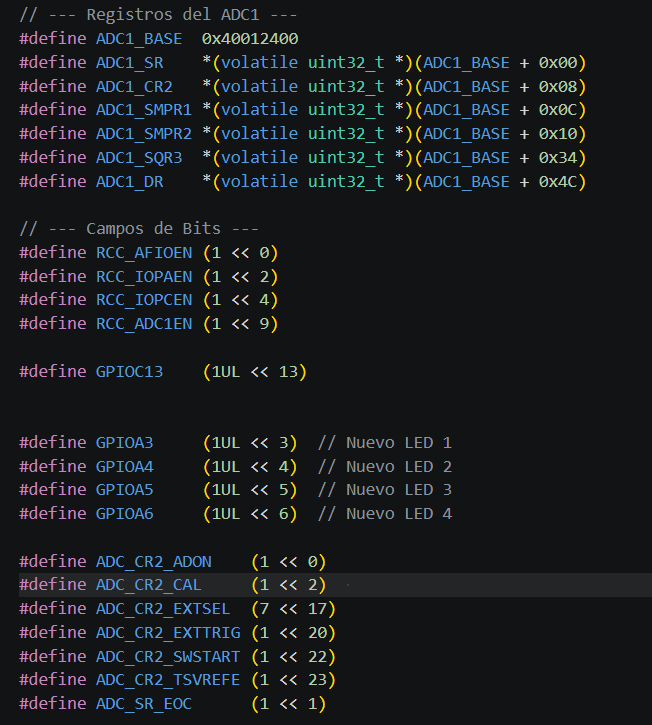
\includegraphics[width=0.4\textwidth]{images/definicionesej2.png}
    \caption*{Definiciones de los registros para interrupciones}
    \label{fig:parte2}
    
\end{figure}

\begin{itemize}
    \item Se definió el registro \textbf{ADC1\_BASE} con la dirección base del ADC, el cual se utiliza para configurar y controlar el funcionamiento del ADC.
    \item Se definió el registro \textbf{ADC1\_SR} el cual se utiliza para verificar el estado del ADC, como por ejemplo si la conversión ha terminado o si hay algún error.
    \item Se definió el registro \textbf{ADC\_CR2} el cual se utiliza para configurar el ADC, como por ejemplo habilitar el ADC, configurar el modo de conversión, etc.
    \item Se definió el registro \textbf{ADC\_SMPR1} el cual se utiliza para configurar el tiempo de muestreo del ADC, lo cual es importante para obtener una conversión precisa.
    \item Se definió el registro \textbf{ADC\_SMPR2} el cual se utiliza para configurar el tiempo de muestreo del ADC para los canales 0 a 9.
    \item Se definió el registro \textbf{ADC\_SQR3} el cual se utiliza para configurar el canal que se va a convertir.
    \item Se definió el registro \textbf{ADC\_DR} el cual se utiliza para leer el resultado de la conversión del ADC.
\end{itemize}

Luego se configuró que al presionar el botón se cambie el canal del ADC entre el potenciómetro y el sensor de temperatura, para esto se configuró una interrupción externa en el pin PA2, la cual se activa al detectar un flanco de subida. En la rutina de servicio de interrupción se cambia el canal del ADC entre el potenciómetro y el sensor de temperatura.

\begin{figure}[H]
    \centering
    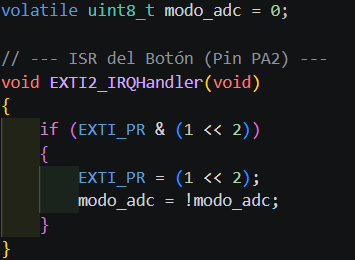
\includegraphics[width=0.5\textwidth]{images/conmutado.png}
    \caption*{Diagrama de conexiones para el ejercicio 2}
    \label{fig:parte2_2}
\end{figure}

Ahora lo nuevo que se implementa es el conversor ADC, el cual se inicializa de la siguiente forma:

\begin{figure}[H]
    \centering
    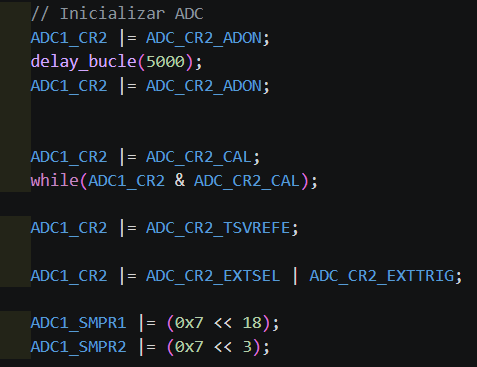
\includegraphics[width=0.45\textwidth]{images/inicializarADC.png}
    \caption*{Inicialización del ADC}
    \label{fig:parte2_3}
\end{figure}

Ahora se programa la función main en la cual se programa de que PIN se leerá el valor del ADC, y se muestra el resultado en los leds. 

\begin{figure}[H]
    \centering
    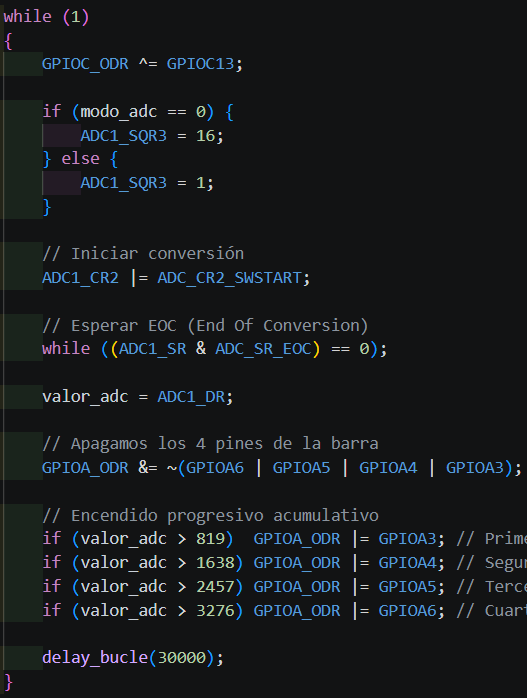
\includegraphics[width=0.45\textwidth]{images/mainej2.png}
    \caption*{Función main para el ejercicio 2}
    \label{fig:parte2_4}
\end{figure}

\begin{itemize}
    \item Se configuró el registro \textbf{ADC1\_SQR3} es el registro de Secuencia Regular 3. Aqui le estamos diciendo al microcontrolador qué canal físico debe conectar al núcleo del ADC en este momento. Si es 1 lee el PA1 y si es 16 lee el sensor de temperatura interno.
    \item Se configuró el registro \textbf{ADC1\_CR2} el cual es Registro de Control 2 del ADC y es donde se configura su comportamiento. Al operar este registro con \textbf{ADC\_CR2\_SWSTART} (SoftWare Start) estamos haciendo que lea voltaje en ese momento.
    \item Polling es el término que se utiliza cunado se configura una espera bloqueante para que se pueda realizar la conversión. Dentro del while se encuentra \textbf{ADC1\_SR \& ADC\_SR\_EOC}, el cual opera El registro de estado del ADC con el bit de fin de conversión (EOC). Mientras se está realizando la conversión el bit EOC se mantiene en 0, y cuando la conversión termina el bit EOC se pone en 1.
    \item \textbf{Encendido progresivo de leds} en esta cadena de if se va encendiendo un led cada vez que el valor del ADC supera un umbral específico. Por ejemplo, si el valor del ADC es mayor a 819, se enciende el primer led, si es mayor a 1638 se enciende el segundo led, y así sucesivamente.
\end{itemize}

\begin{figure}[H]
    \centering
    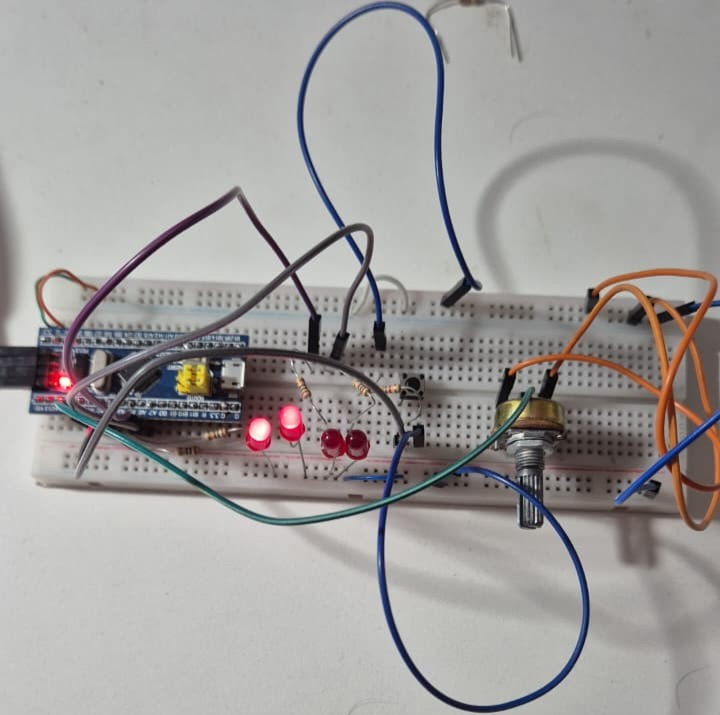
\includegraphics[width=0.4\textwidth]{images/proto2a.jpeg}
    \caption*{Funcionamiento sensor de temperatura}
    \label{fig:parte2_5}
\end{figure}

\begin{figure}[H]
    \centering
    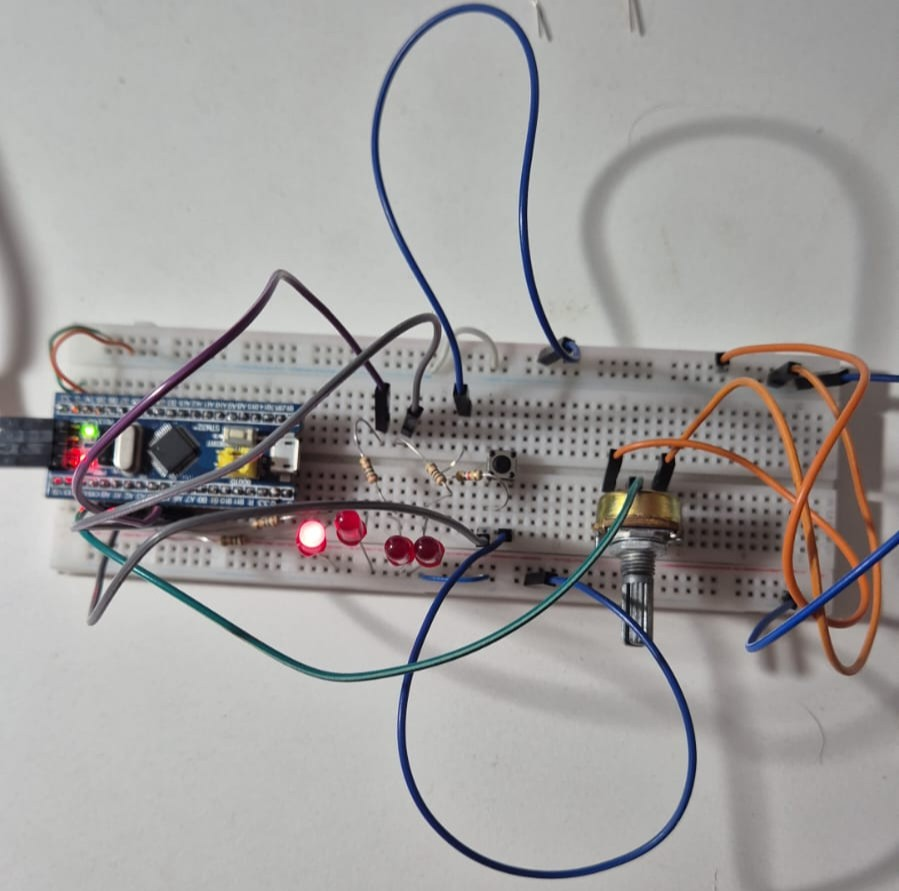
\includegraphics[width=0.4\textwidth]{images/proto2b.jpeg}
    \caption*{Funcionamiento potenciómetro con valor bajo de voltaje}
    \label{fig:parte2_6}
\end{figure}

\begin{figure}[H]
    \centering
    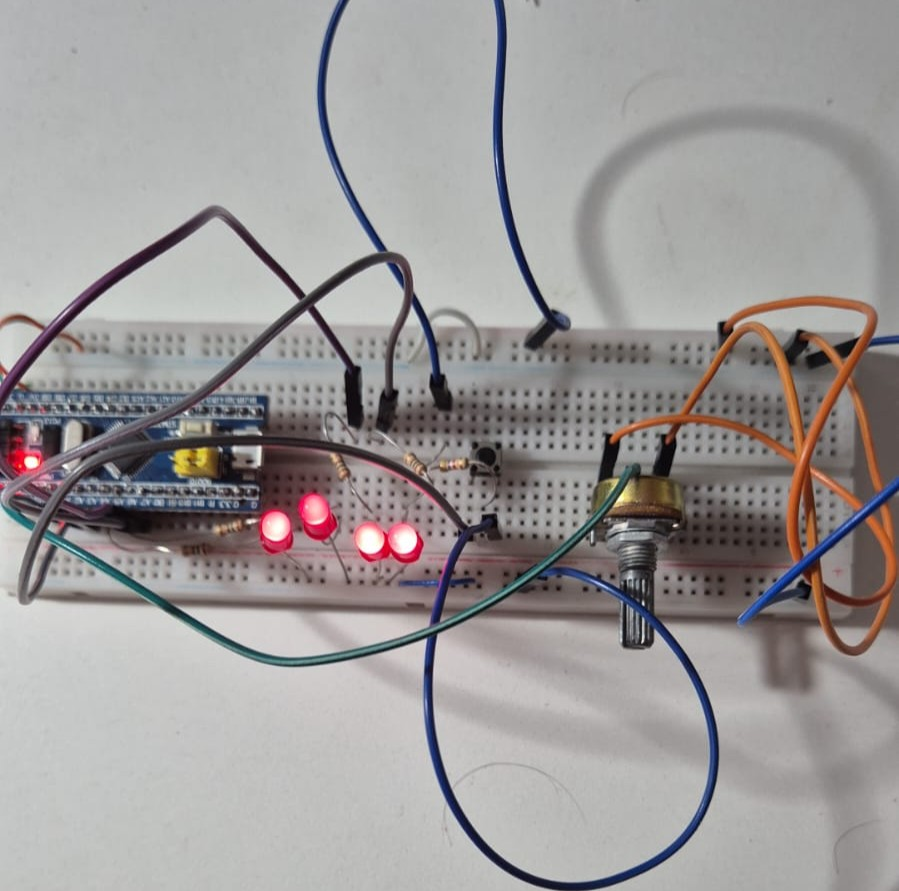
\includegraphics[width=0.4\textwidth]{images/proto2c.jpeg}
    \caption*{Funcionamiento potenciómetro con valor alto de voltaje}
    \label{fig:parte2_7}
\end{figure}

La primera imagen corresponde a la lectura del sensor de temperatura, como esta es media respecto al rango de lectura del ADC, se encienden solamente dos leds. La segunda imagen corresponde a la lectura del potenciómetro con el valor bajo de volaje, por lo que se enciende solamente un led y la tercera imagen corresponde a la lectura del potenciómetro con el valor alto de volaje, en el cual se encuentran todos los leds encendidos.